%%%%%%%%%%%%%%%%%%%%%%%%%%%%%%%%%%%%%%%%%%%%%%%%%%%%%%%%%%%%%%%%%%%%%%%%%%%%%%%%%%%%%%%%%%%%%%%%%%%%%%%%%%%%%%%%%%%%%%%%%
\subsection{Intuition}
%%%%%%%%%%%%%%%%%%%%%%%%%%%%%%%%%%%%%%%%%%%%%%%%%%%%%%%%%%%%%%%%%%%%%%%%%%%%%%%%%%%%%%%%%%%%%%%%%%%%%%%%%%%%%%%%%%%%%%%%%
\begin{frame}{Intuition}
    \begin{figure}
        \begin{minipage}[t]{0.30\linewidth}
            \centering
            \vspace{0pt}
            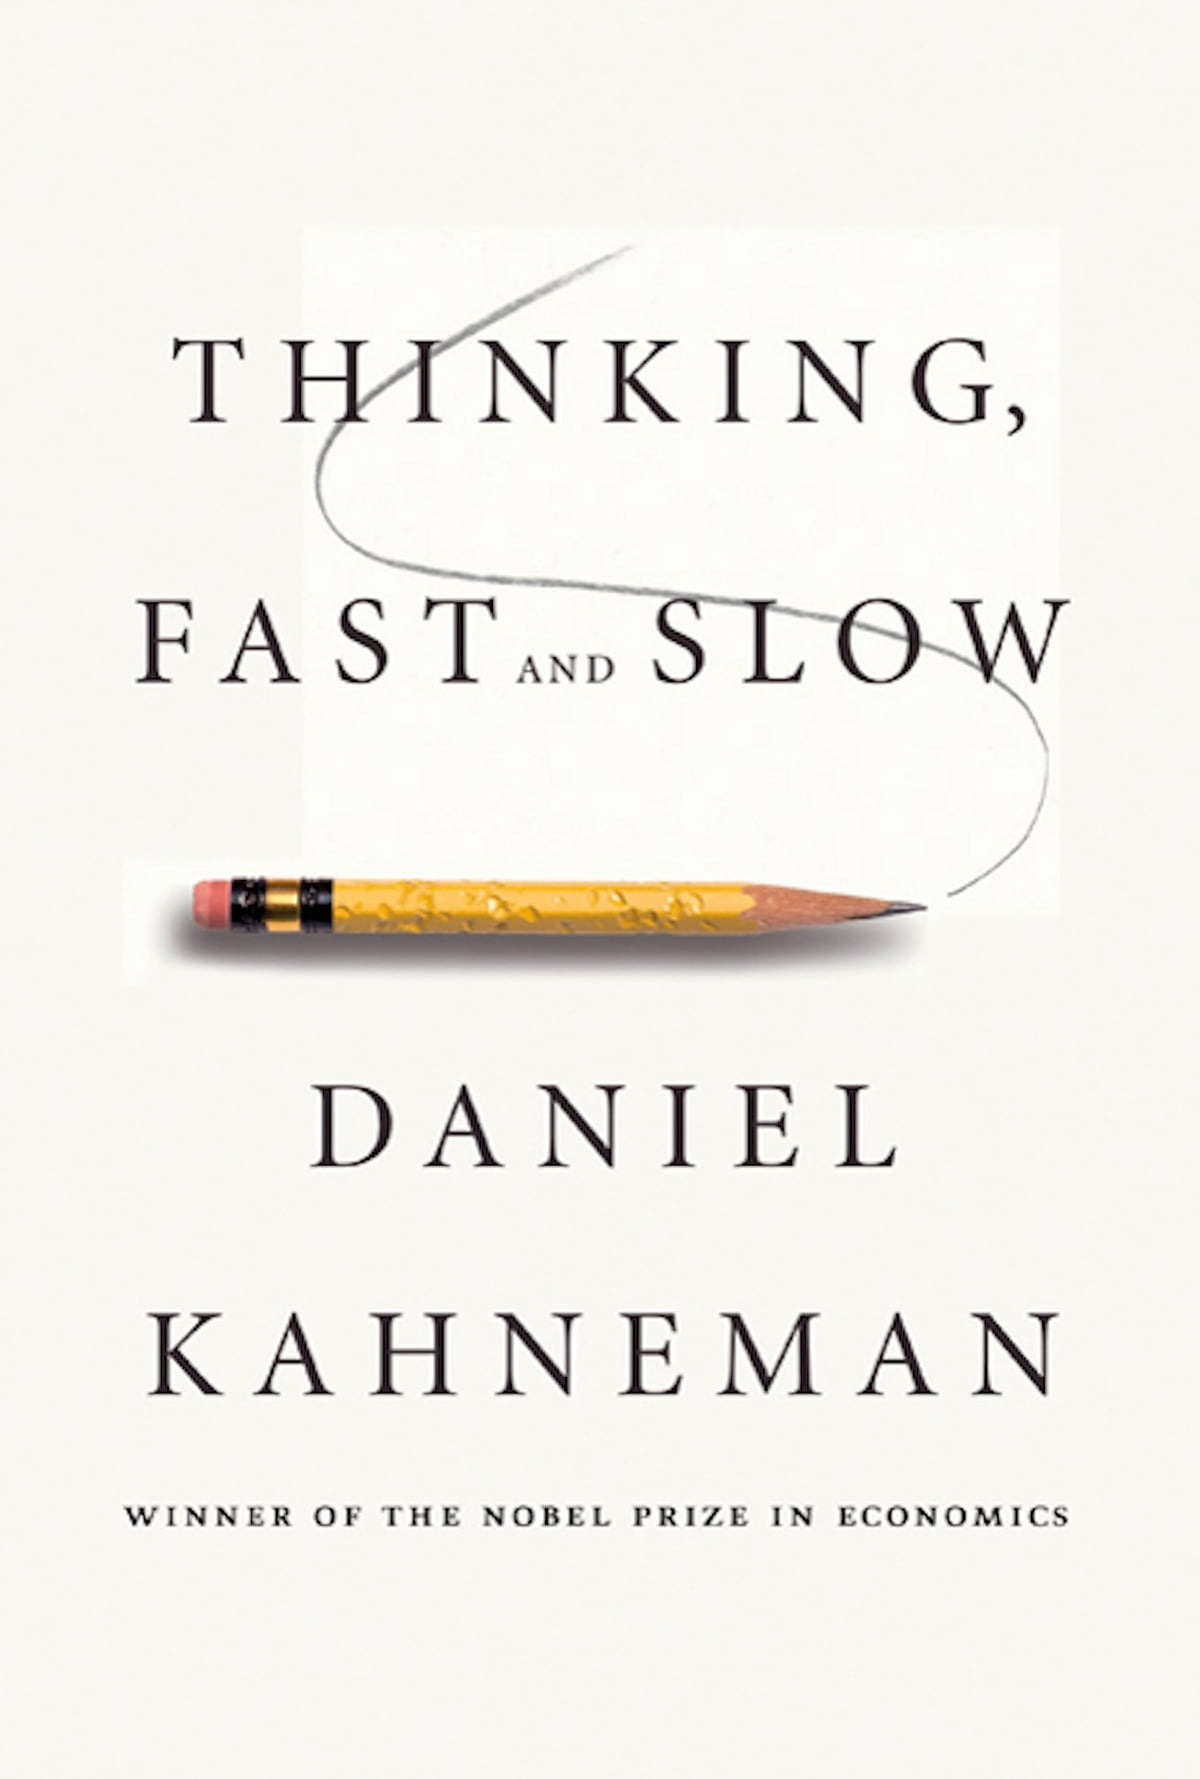
\includegraphics[width=\textwidth]{img/TFS.jpg}
        \end{minipage}
        \hspace{0.5cm}
        \begin{minipage}[t]{0.5\linewidth}
            \vspace{1cm}
            \begin{itemize}
                \item \textbf{Fast Thinking}: Correlation, pattern recognition, subconscious, ...
                \item \textbf{Slow Thinking}: Logical (causal), calculating, conscious, ...
            \end{itemize}
        \end{minipage}
    \end{figure}
    Many researchers believe that AI can only utilize "fast thinking" (System I). They propose causality to reach "slow thinking" (System II).
\end{frame}
%%%%%%%%%%%%%%%%%%%%%%%%%%%%%%%%%%%%%%%%%%%%%%%%%%%%%%%%%%%%%%%%%%%%%%%%%%%%%%%%%%%%%%%%%%%%%%%%%%%%%%%%%%%%%%%%%%%%%%%%%
\subsection{Correlation vs Causation}
%%%%%%%%%%%%%%%%%%%%%%%%%%%%%%%%%%%%%%%%%%%%%%%%%%%%%%%%%%%%%%%%%%%%%%%%%%%%%%%%%%%%%%%%%%%%%%%%%%%%%%%%%%%%%%%%%%%%%%%%%

\begin{frame}{Correlation vs Causation}
    \begin{figure}[t]
        \centering
        \vspace{0pt}
        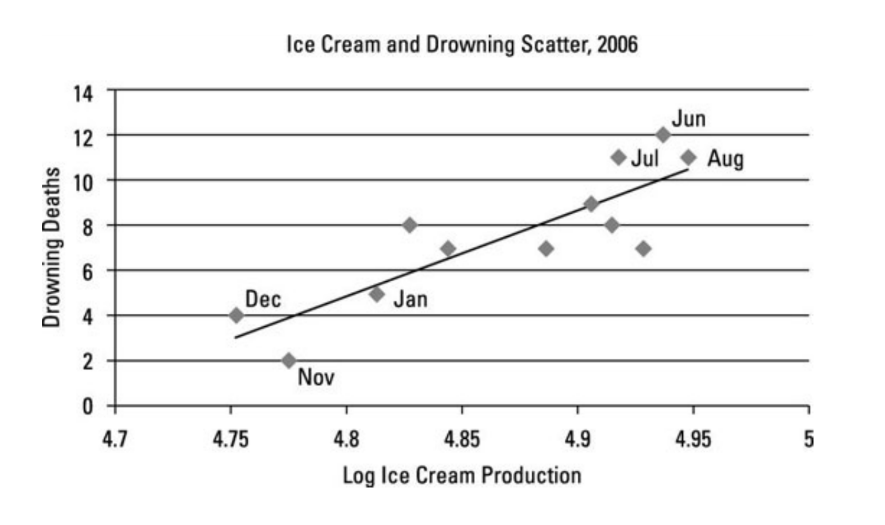
\includegraphics[width=0.7\textwidth]{img/hidden_con.png}
    \end{figure}
    \small{Does ice cream consumption cause drowning? Does the number of drownings cause ice cream cravings from the population?}
    
    \pause
    Of course not, but there is a \textbf{third variable} that causes both: the month of the year. 
\end{frame}
%%%%%%%%%%%%%%%%%%%%%%%%%%%%%%%%%%%%%%%%%%%%%%%%%%%%%%%%%%%%%%%%%%%%%%%%%%%%%%%%%%%%%%%%%%%%%%%%%%%%%%%%%%%%%%%%%%%%%%%%%
\subsection{Interventions}
%%%%%%%%%%%%%%%%%%%%%%%%%%%%%%%%%%%%%%%%%%%%%%%%%%%%%%%%%%%%%%%%%%%%%%%%%%%%%%%%%%%%%%%%%%%%%%%%%%%%%%%%%%%%%%%%%%%%%%%%%
\begin{frame}{Interventions}
    \begin{figure}[t]
        \centering
        \vspace{0pt}
        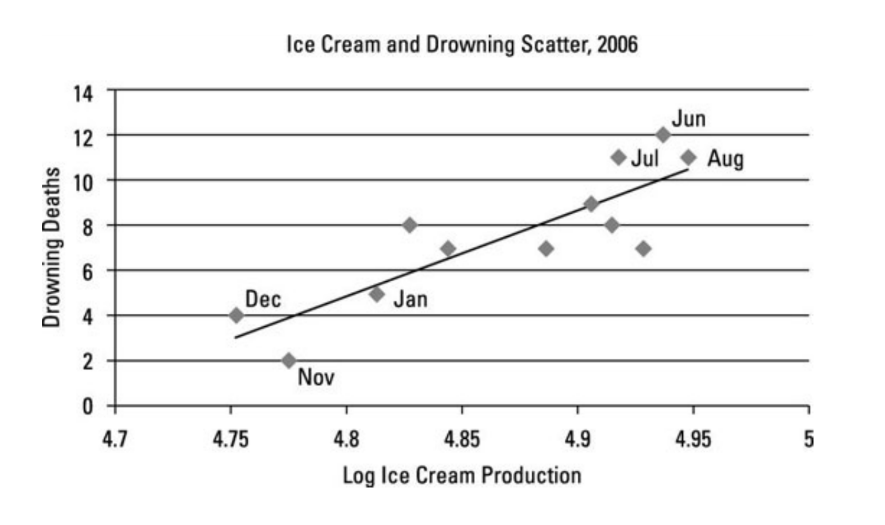
\includegraphics[width=0.7\textwidth]{img/hidden_con.png}
    \end{figure}
    But how can we know if two correlated events have a cause-effect structure? 
    \pause

    By using \textbf{interventions!}

    (e.g. If we force people to randomly eat ice cream, we will see that the number of drownings stays the same.)
\end{frame}
    